\section{Introduction}\label{sec:intro}

\subsection{Problem Background}

The carbon cycle describes the process of the exchange of carbon throughout the geochemical cycle of the Earth, and is a vital component for life on the planet. One key component of this part of the process is the decomposition of plant material and woody fibers.

Some of the key agents in decomposing woody fibers are fungi. The authors of a recent research article on wood decomposition by fungi identified fungi traits that determine decomposition rates and also noted links between certain traits. In particular, the slow growing strains of fungi tend to be better able to survive and grow in the presence of environmental changes with respect to moisture and temperature, while the faster growing strains tend to be less robust to the same changes.

\subsection{Problem Restatement}
\begin{itemize}
\item Build a mathematical model that describes the breakdown of ground litter and woody fibers through fungal activity in the presence of multiple species of fungi.
\item In the mathematical model, incorporate the interactions between different species of fungi, which have different growth rates and different moisture tolerances.
\item Provide an analysis of the model and describe the interactions between the different types of fungi. The dynamics of the interactions should be characterized and described including both short- and long-term trends. The analysis should examine the sensitivity to rapid fluctuations in the environment, and should determine the overall impact of changing atmospheric trends to assess the impact of variation of local weather patterns.
\item Include predictions about the relative advantages and disadvantages for each species and combinations of species likely to persist, and do so for different environments including arid, semi-arid, temperate, arboreal, and tropical rain forests.
\item Describe how the diversity of fungal communities of a system impacts the overall efficiency of a system with respect to the breakdown of ground litter. Predict the importance and role of biodiversity in the presence of different degrees of variability in the local environment.
\end{itemize}
\subsection{Our Work}

\begin{figure}\caption{Work flow of our modelling}
    \begin{center}
        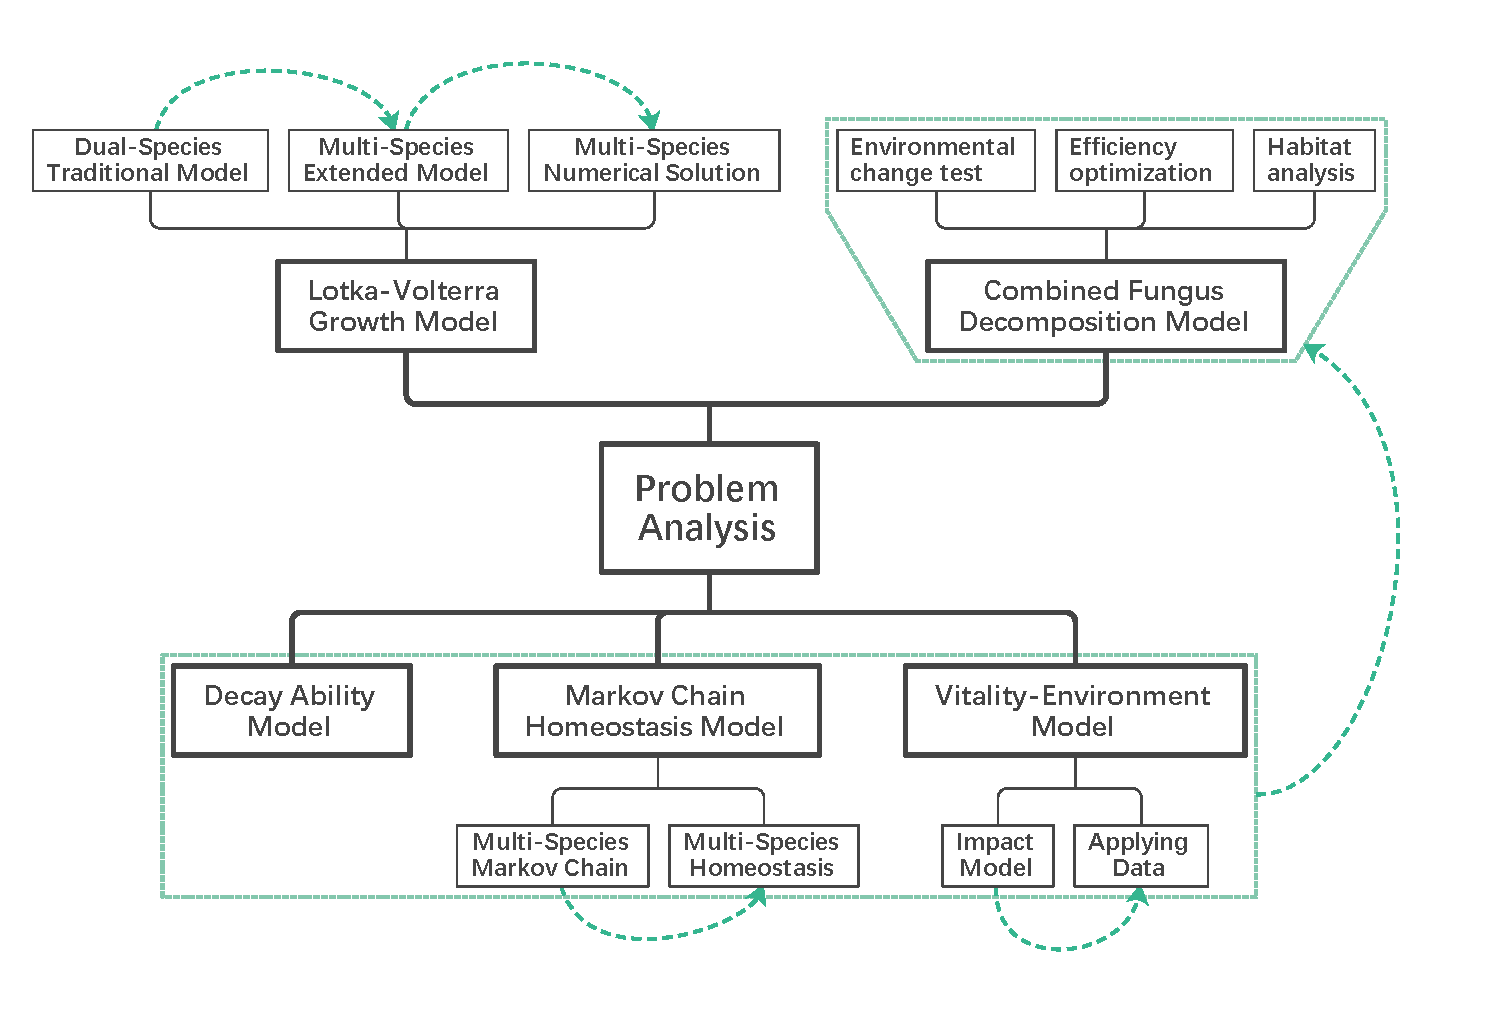
\includegraphics[width=\columnwidth]{workflow.pdf}
    \end{center}\end{figure}
